\chapter{Gravitational Field}

\section{Gravitational Force and Field}

\begin{definition}
    A \vocab{gravitational field} is a region of space within which a mass experiences a gravitational force.
\end{definition}

A gravitational field can be represented by directed lines of force.

\begin{law}[Newton's Law of Gravitation]
    Two point masses attract each other with a force that is proportional to the product of their masses and inversely proportional to the square of their separation. Mathematically, \[F = \frac{G m_1 m_2}{r^2},\] where $G = 6.67 \times 10^{-11}$ N m$^2$ kg$^{-2}$ is the constant of proportionality known as the \vocab{gravitational constant}.
\end{law}

Note that point masses have non-zero mass and no volume. If two objects are placed sufficiently far apart such that their dimensions become negligible compared to the distance separating them, the two objects can be considered point masses.

\begin{definition}
    The \vocab{gravitational field strength} ($g$) at a point is the gravitational force per unit mass exerted on a small test mass placed at that point. \[g = \frac{F}{m}.\]
\end{definition}

$g$ is a vector quantity. It is in the same direction as the gravitational force. Its SI unit is newtons per kilogram (N kg$^{-1}$).

\begin{proposition}
    The gravitational field strength $g$ at a point a distance $r$ measured from a point mass $M$ is given by \[g = \frac{GM}{r^2}.\]
\end{proposition}
\begin{proof}
    Consider two point masses $M$ and $m$ separated by a distance $r$. By Newton's law of gravitation, the magnitude of the attractive gravitational force $F$ acting on the mass $m$ due to the gravitational field of $M$ is given by \[F = \frac{GMm}{r^2}.\] Based on the definition of gravitational field strength, the magnitude of $g$ at the point where $m$ is situated is hence \[g = F/m = \frac{GM}{r^2}.\]
\end{proof}

\section{Gravitational Potential Energy}

\begin{definition}
    The \vocab{gravitational potential energy} (GPE, $U$) of a mass at a point is the work done on the mass in moving it from infinity to that point.
\end{definition}

\begin{proposition}
    The gravitational potential energy of a mass $m$ at a distance $r_0$ from a mass $M$ is given by \[U = -\frac{GMm}{r_0}.\]
\end{proposition}
\begin{proof}
    Recall that \[F = -\der{U}{r}.\] Hence, \[U = -\int_{\infty}^{r_0} F \d r = -\int_\infty^{r_0} \frac{GMm}{r^2} \d r = -\frac{GMm}{r_0}.\]
\end{proof}

\begin{definition}
    The \vocab{gravitational potential} ($\f$) at a point is the work done per unit mass in bringing a small test mass from infinity to that point. Mathematically, \[\f = \frac{U}{m}.\]
\end{definition}

Gravitational potential is a scalar quantity. Its SI unit is joules per kilogram (J kg$^{-1}$).

\begin{proposition}
    The potential at a distance $r$ away from a point mass $M$ is given by \[\f = -\frac{GM}{r}.\]
\end{proposition}
\begin{proof}
    Recall that $U = -GMm/r$. By the definition of gravitational potential, \[\f = \frac{U}{m} = -\frac{GM}{r}.\]
\end{proof}

\begin{definition}
    The \vocab{potential gradient} in a gravitational field is the change in gravitational potential per unit displacement in the direction of the field. Mathematically, \[\text{potential gradient} = \der{\f}{r}.\]
\end{definition}

Potential gradient is a vector quantity. Its SI unit is joules per kilogram per metre (J kg$^{-1}$ m$^{-1}$).

\begin{proposition}
    The field strength $g$ of a gravitational field at a point is numerically equal but opposite in direction to the potential gradient at that point. Mathematically, \[g = -\der{\f}{r}.\]
\end{proposition}
\begin{proof}
    By the definition of $g$ and $\f$, we see that \[g = \frac{F}{m} = - \frac1m \der{U}{r} = -\der{(U/m)}{r} = -\der{\f}{r}.\]
\end{proof}

The below figure summarizes the relationships between $F$, $U$, $g$ and $\f$.

\begin{figure}[H]
    \centering
    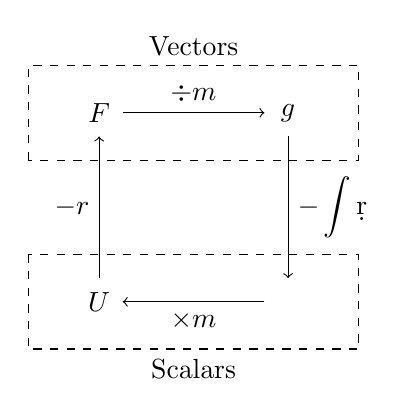
\begin{tikzpicture}[scale=0.6]
        \node at (-2, 2) {$F$};
        \node at (2, 2) {$g$};
        \node at (-2, -2) {$U$};
        \node at (2, -2) {$\f$};

        \draw[->] (-1.5, 2) -- (1.5, 2);
        \node[anchor=south] at (0, 2) {$\div m$};

        \draw[->] (1.5, -2) -- (-1.5, -2);
        \node[anchor=north] at (0, -2) {$\times m$};

        \draw[->] (2, 1.5) -- (2, -1.5);
        \node[anchor=west] at (2, 0) {$\displaystyle -\int \d r$};

        \draw[->] (-2, -1.5) -- (-2, 1.5);
        \node[anchor=east] at (-2, 0) {$\displaystyle -\der{}{r}$};

        \draw[dashed] (-3.5, 1) rectangle (3.5, 3);
        \draw[dashed] (-3.5, -1) rectangle (3.5, -3);

        \node[anchor=south] at (0, 3) {Vectors};
        \node[anchor=north] at (0, -3) {Scalars};
    \end{tikzpicture}
    \caption{A summary of gravitational fields.}
\end{figure}

\section{Orbital Motion}

\subsection{Circular Orbits}

\begin{law}
    For an object in a circular orbit of radius $r$, the square of its orbital period $T$ is proportional to the cube of the radius.
\end{law}
\begin{proof}
    Suppose object A (of mass $m$) is in circular orbit around object $B$ (of mass $M$). Let $T$ be the orbital period and let $r$ be the distance between A and B.

    A is in circular motion. The gravitational force acting on A by B provides the centripetal force. Hence, \[\frac{GMm}{r^2} = mr\o^2.\] Since $\o = 2\pi/T$, we obtain \[\frac{GMm}{r^2} = \frac{4\pi^2 mr}{T^2} \implies T^2 = \frac{4\pi^2}{GM} r^3,\] so $T^2 \propto r^3$.
\end{proof}

\begin{proposition}
    The kinetic energy of an orbiting mass $m$ is given by \[E_k = \frac{GMm}{2r}.\]
\end{proposition}
\begin{proof}
    Like above, we observe that the gravitational force on the mass provides the centripetal force, so \[\frac{GMm}{r^2} = \frac{mv^2}{r} \implies E_k = \frac12 mv^2 = \frac{GMm}{2r}.\]
\end{proof}

\begin{corollary}
    The mechanical energy of an orbiting mass $m$ is given by \[E_{\text{total}} = -\frac{GMm}{2r} = -E_k.\]
\end{corollary}
\begin{proof}
    Recall that the mechanical energy is the sum of the mass's KE and GPE. Hence, \[E_{\text{total}} = E_k + E_p = \frac{GMm}{2r} + \bp{- \frac{GMm}{r}} = -\frac{GMm}{2r}.\]
\end{proof}

Paradoxically, if the total energy of the orbiting mass increases, its kinetic energy must \emph{decrease}. However, the process of increasing the total energy is typically started by \emph{increasing} its speed! This paradox arises because $E_k \propto 1/r$; any increase in total must necessarily increase $r$, which results in a decrease in kinetic energy, and vice versa.

\subsection{Geostationary Orbits}

\begin{definition}
    A \vocab{geostationary orbit} is a circular orbit around the Earth on which an orbiting mass would appear stationary to an observer on the Earth's surface.
\end{definition}

For an object to be in geostationary orbit, it must satisfy the following conditions:
\begin{itemize}
    \item it must be in equatorial orbit (vertically above the equator);
    \item it must have an orbital period of 24 hours; and
    \item it must move from west to east.
\end{itemize}